%\documentclass[gray,handout, pdftex, 11pt]{beamer}
%\documentclass[handout, pdftex, 11pt]{beamer}
\documentclass[pdftex, 11pt]{beamer}

\usepackage{pgfpages}
\usepackage[utf8]{inputenc}
\usepackage[T1]{fontenc}
\usepackage{lmodern}
%\usepackage[italian]{babel}
\usepackage{graphicx}
\usepackage{microtype}
\usepackage{acronym}
\usepackage{array}
%\usepackage{natbib}

\usepackage{tikz}
\usetikzlibrary{intersections, arrows, shapes, decorations.pathreplacing, decorations.pathmorphing, calc}

\usepackage{appendixnumberbeamer}

\mode<presentation>{
  %-------------------------1
  \usetheme{Boadilla}
  \usecolortheme{beaver}
  %-------------------------1
  %-------------------------2
  %\usetheme{Goettingen}
  %\usecolortheme{sidebartab}
  %-------------------------2
  %\useoutertheme[right]{sidebar}
  %\usefonttheme{default}
  \setbeamercovered{transparent}
  %\setbeameroption{show notes on second screen=right}
  \setbeamertemplate{navigation symbols}{}

  \bibliographystyle{abbrv}  
  %\renewcommand\bibfont{\scriptsize}
  \setbeamertemplate{bibliography item}{\textbullet}
  \setbeamertemplate{itemize item}{\checkmark}
  \setbeamertemplate{itemize subitem}{-}
  \setbeamertemplate{enumerate items}[default]
  \setbeamertemplate{sections/subsections in toc}[square]
}

%stili
\tikzstyle{linea}=[draw, green]
\tikzstyle{service}=[very thick, draw, blue]
\tikzstyle{newService}=[very thick, draw, red]
\tikzstyle{modulo}=[thick, draw, black]
\tikzstyle{freccia}=[->, very thick, >=stealth', draw, red]


\newcommand{\frecciadx}{~{\tikz[baseline] \draw[freccia] (0,0.5ex) --
  (5.5ex,0.5ex);}~}

\title[Upgrade of material model in TkLayout]{\textbf{Status and testing of the upgrade of material model in TkLayout}}
\subtitle{Tracker Week}
\institute[CERN]{
  %{\Large\textbf{CERN}}\\{European Organization for Nuclear Research}\\[0.5cm]
  %\\[0.2cm]
  European Organization for Nuclear Research\\[0.5cm]
  
\includegraphics[width=2cm]{img/LogoBadge.pdf}\\
}

\author[Stefano Martina]{
  %\\[0.2cm]
  \textbf{Stefano MARTINA}\\
  {\small stefano.martina@cern.ch}
}

\date[\today]{\flushright \today}

\begin{document}

\begin{frame}[plain,noframenumbering]
  \titlepage
\end{frame}

\begin{frame}{Old model}
  \begin{center}
    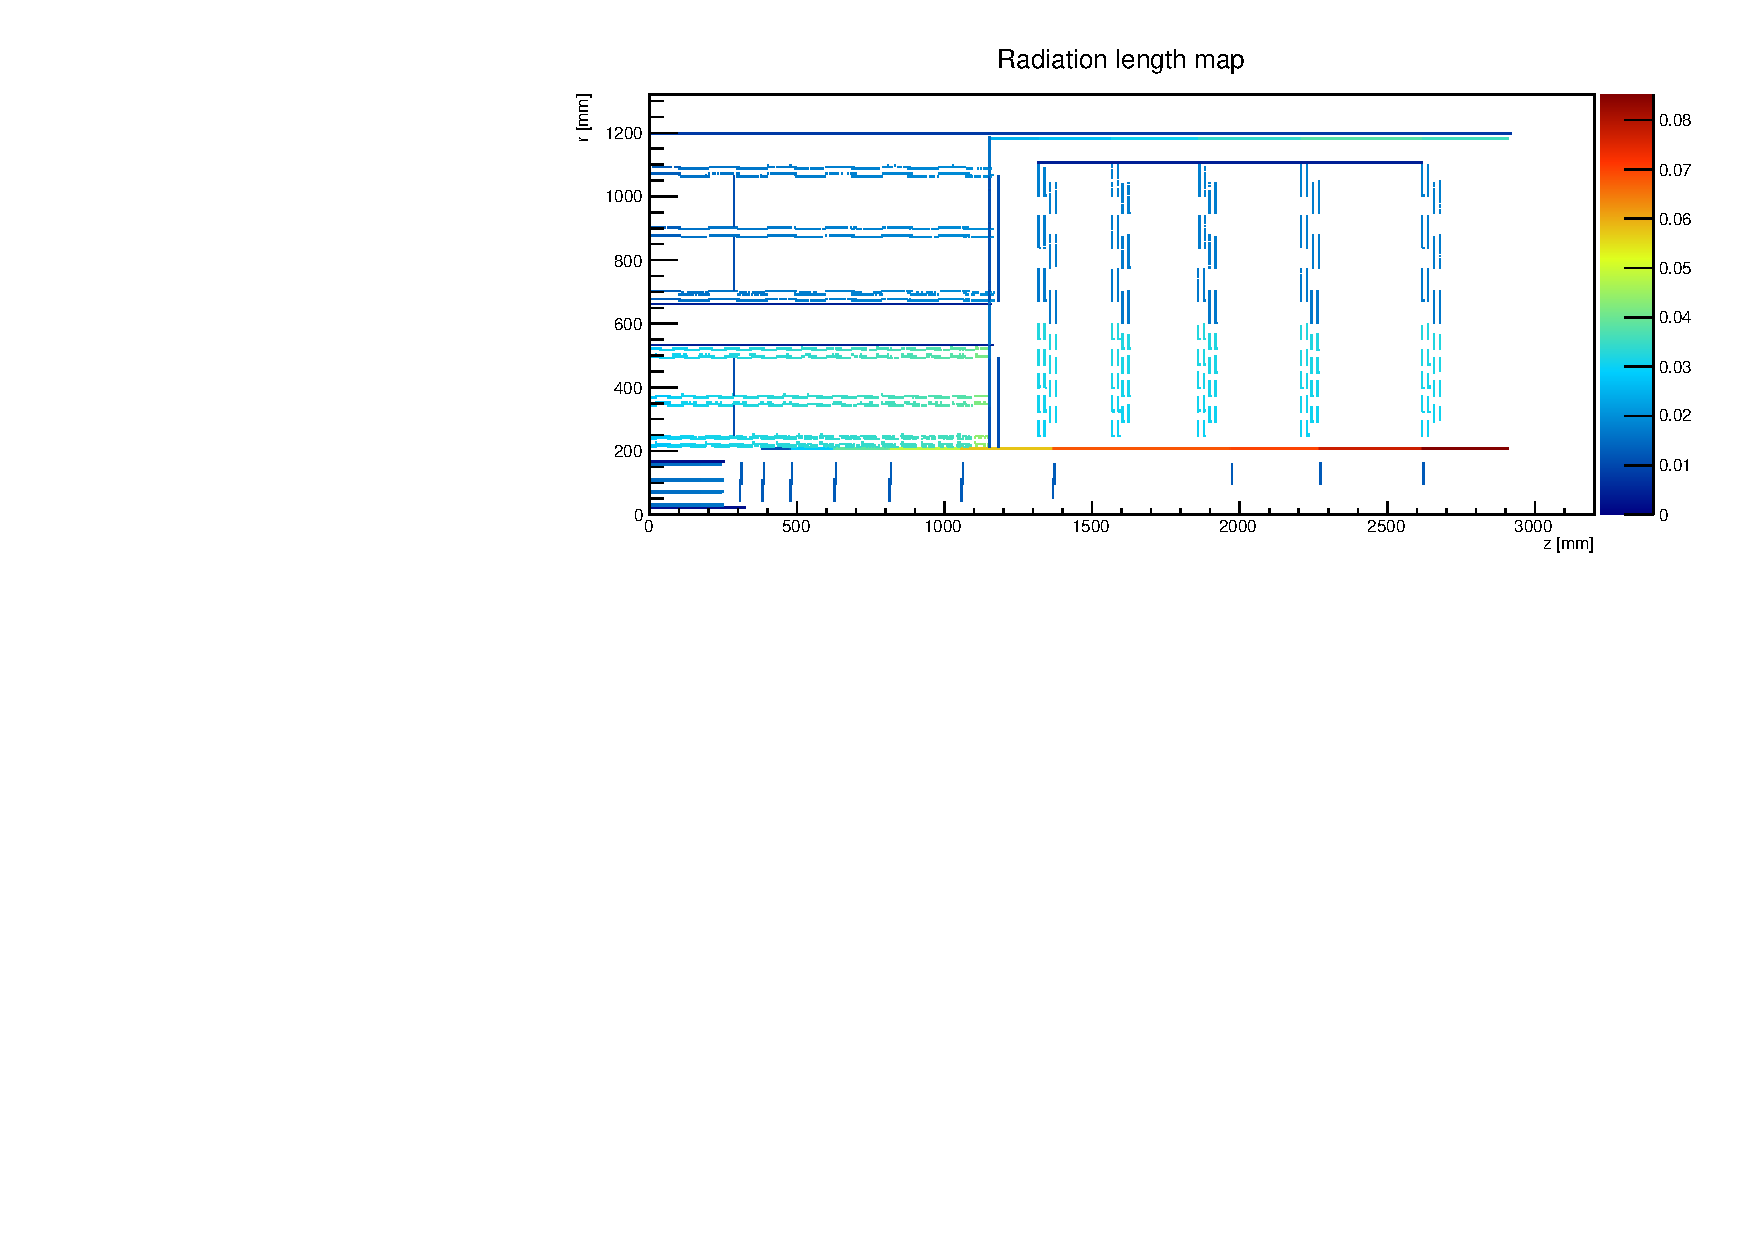
\includegraphics[width=\textwidth]{img/oldModel.pdf}
  \end{center}
  \begin{itemize}
  \item Cables material distributed \alert{inside} modules volumes
  \item Possible to model \alert{cooling pipe} along rods, \alert{manifold} in the flange and bigger cooling pipe out of the barrel
  \end{itemize}
\end{frame}

\begin{frame}{New model}
  \begin{center}
    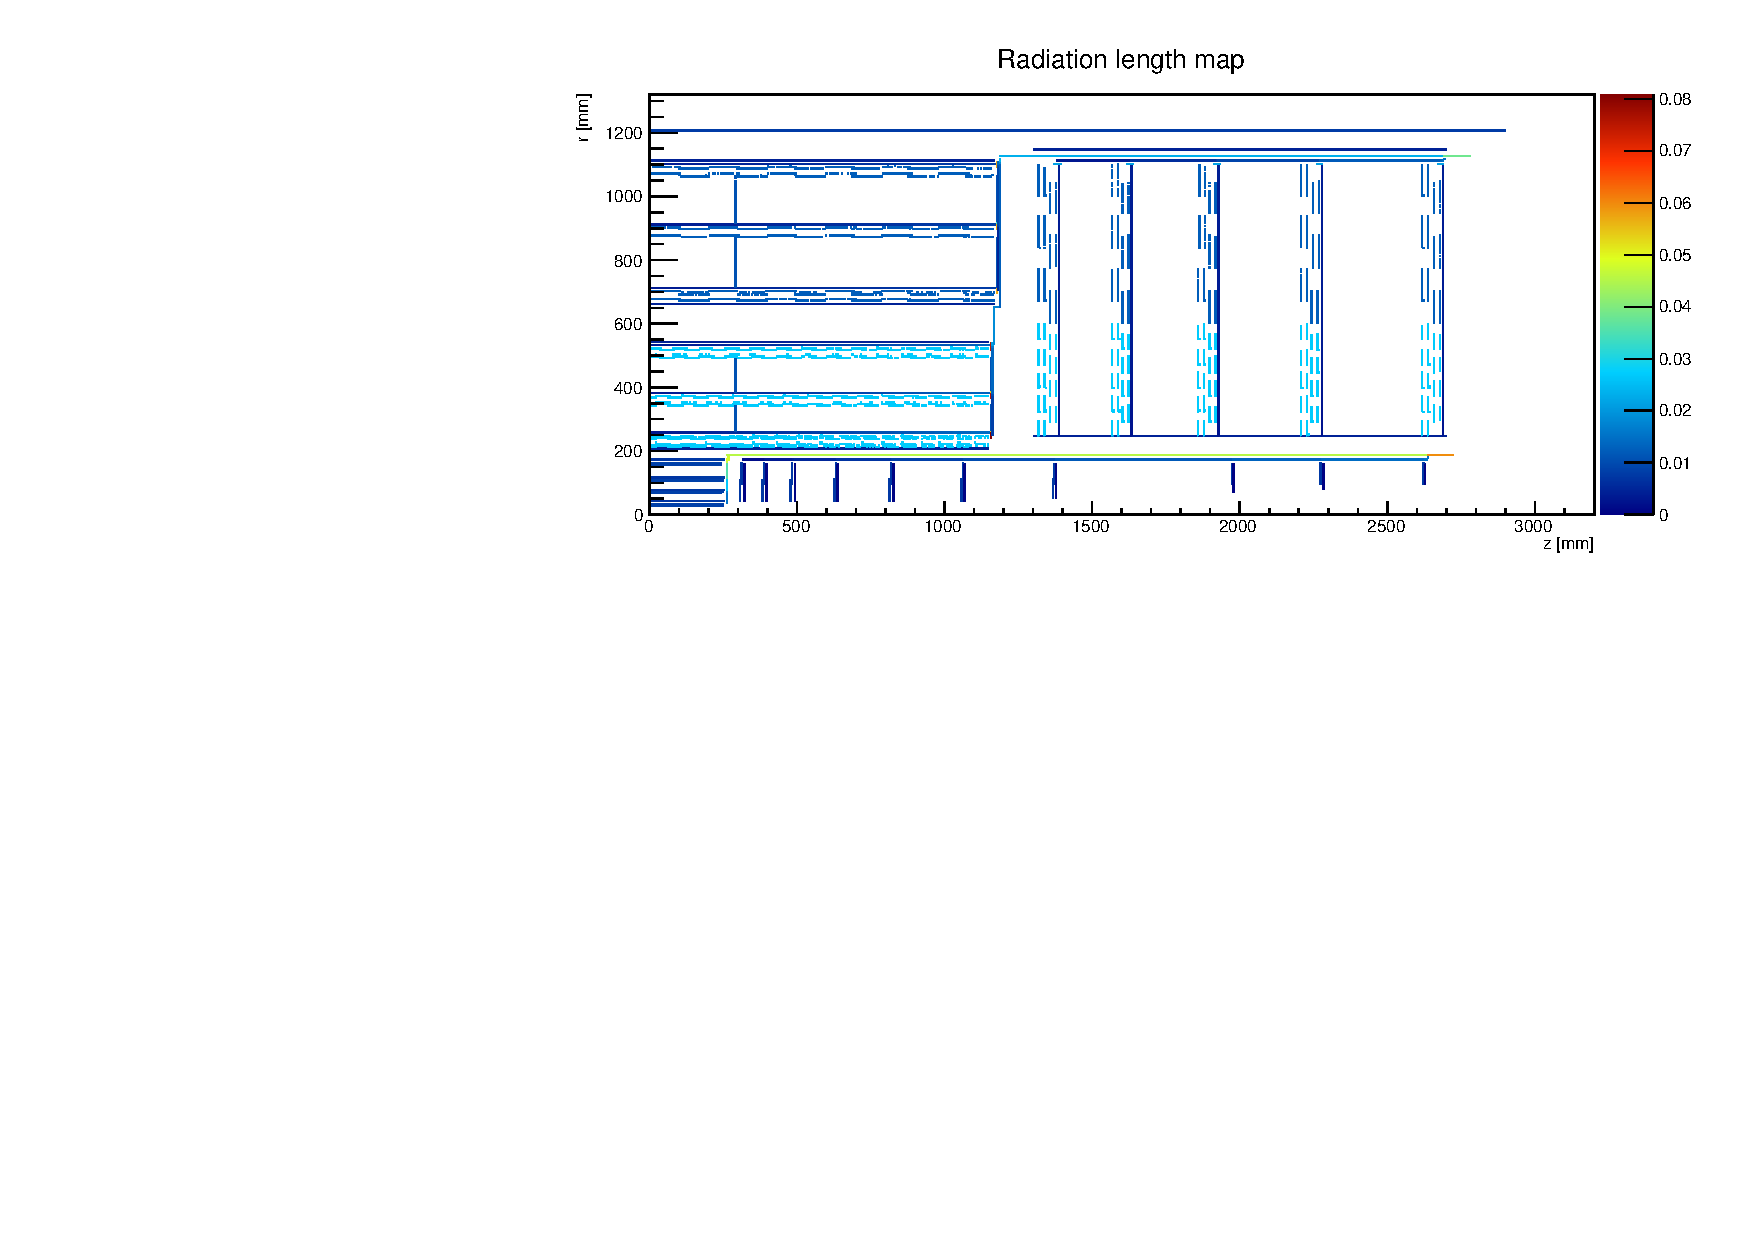
\includegraphics[width=\textwidth]{img/newModel.pdf}
  \end{center}
  \begin{itemize}
  \item Cables material in \alert{dedicated} volumes
  \item More \alert{detailed}
  \item Better routing \alert{algorithm}
  \item More \alert{functionalities}
  \end{itemize}
\end{frame}

\begin{frame}{Advantages}
  \begin{block}{Correct description for \alert{tilted} modules}
    \begin{itemize}
    \item In old model the cables were distributed \alert{over} the modules
      \begin{itemize}
      \item \alert{Not} feasible in case of tilted modules
      \end{itemize}
    \item Now is \alert{possible} to model this design
    \end{itemize}
  \end{block}
  \begin{center}
    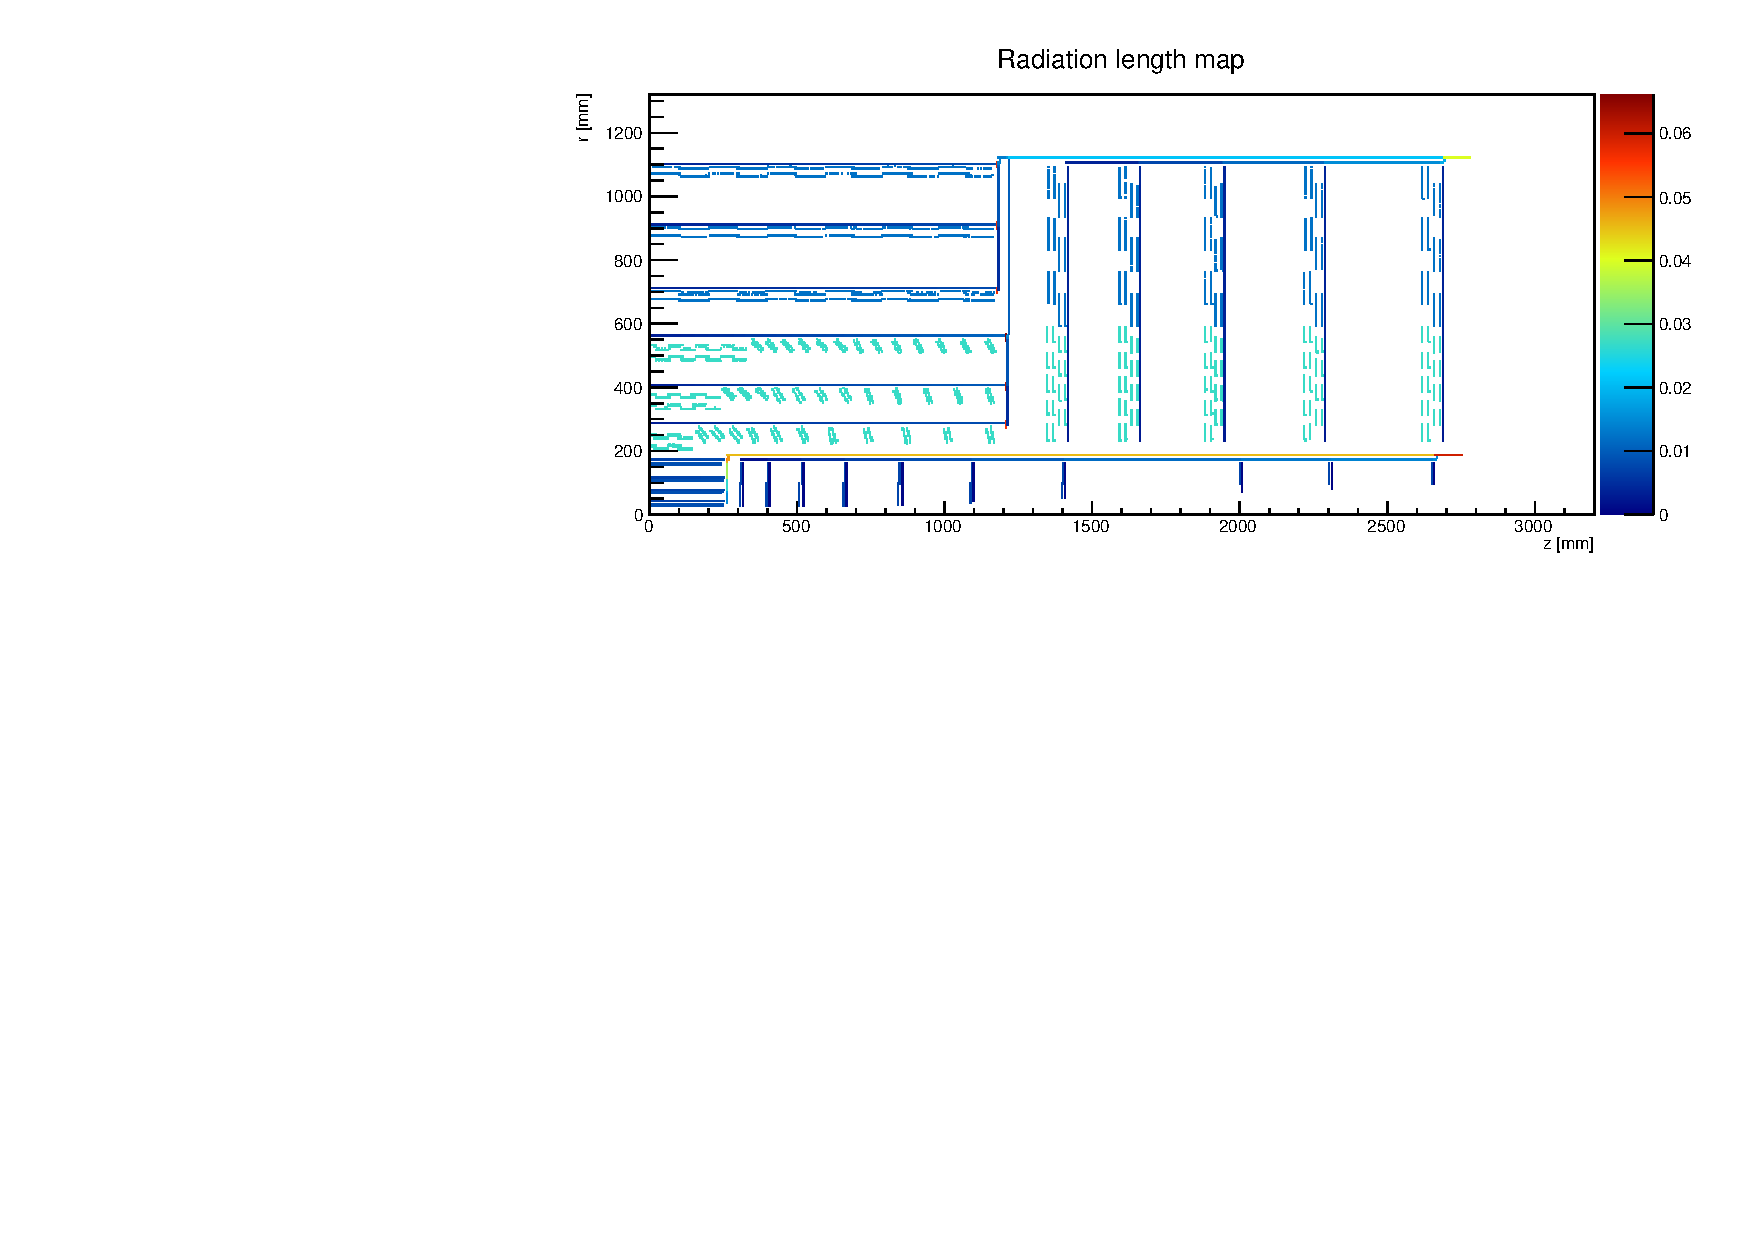
\includegraphics[width=\textwidth]{img/tilted.pdf}
  \end{center}
\end{frame}

\begin{frame}{New feature}
  \begin{block}{Model for \alert{pixel-like} materials}
    \begin{itemize}
    \item For instance \alert{twisted pair} from modules, electrical optical \alert{transducer}, and \alert{optic fibers} after it
    \end{itemize}
  \end{block}
  \begin{center}
    \only<1>{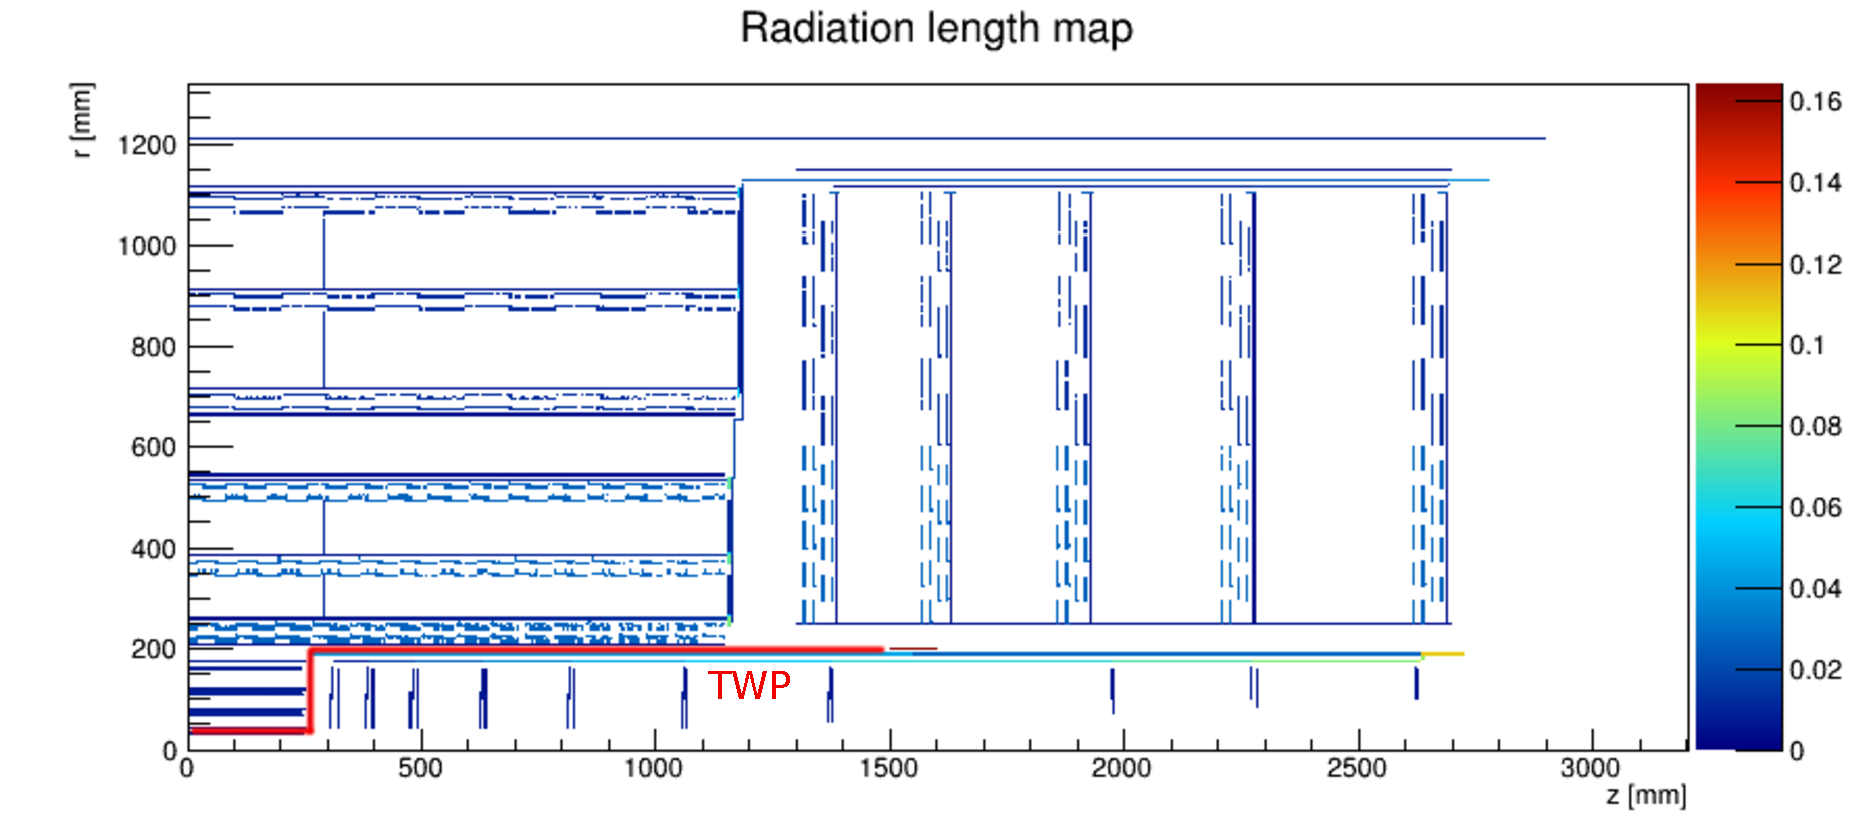
\includegraphics[width=\textwidth]{img/electro-opto1.pdf}}
    \only<2>{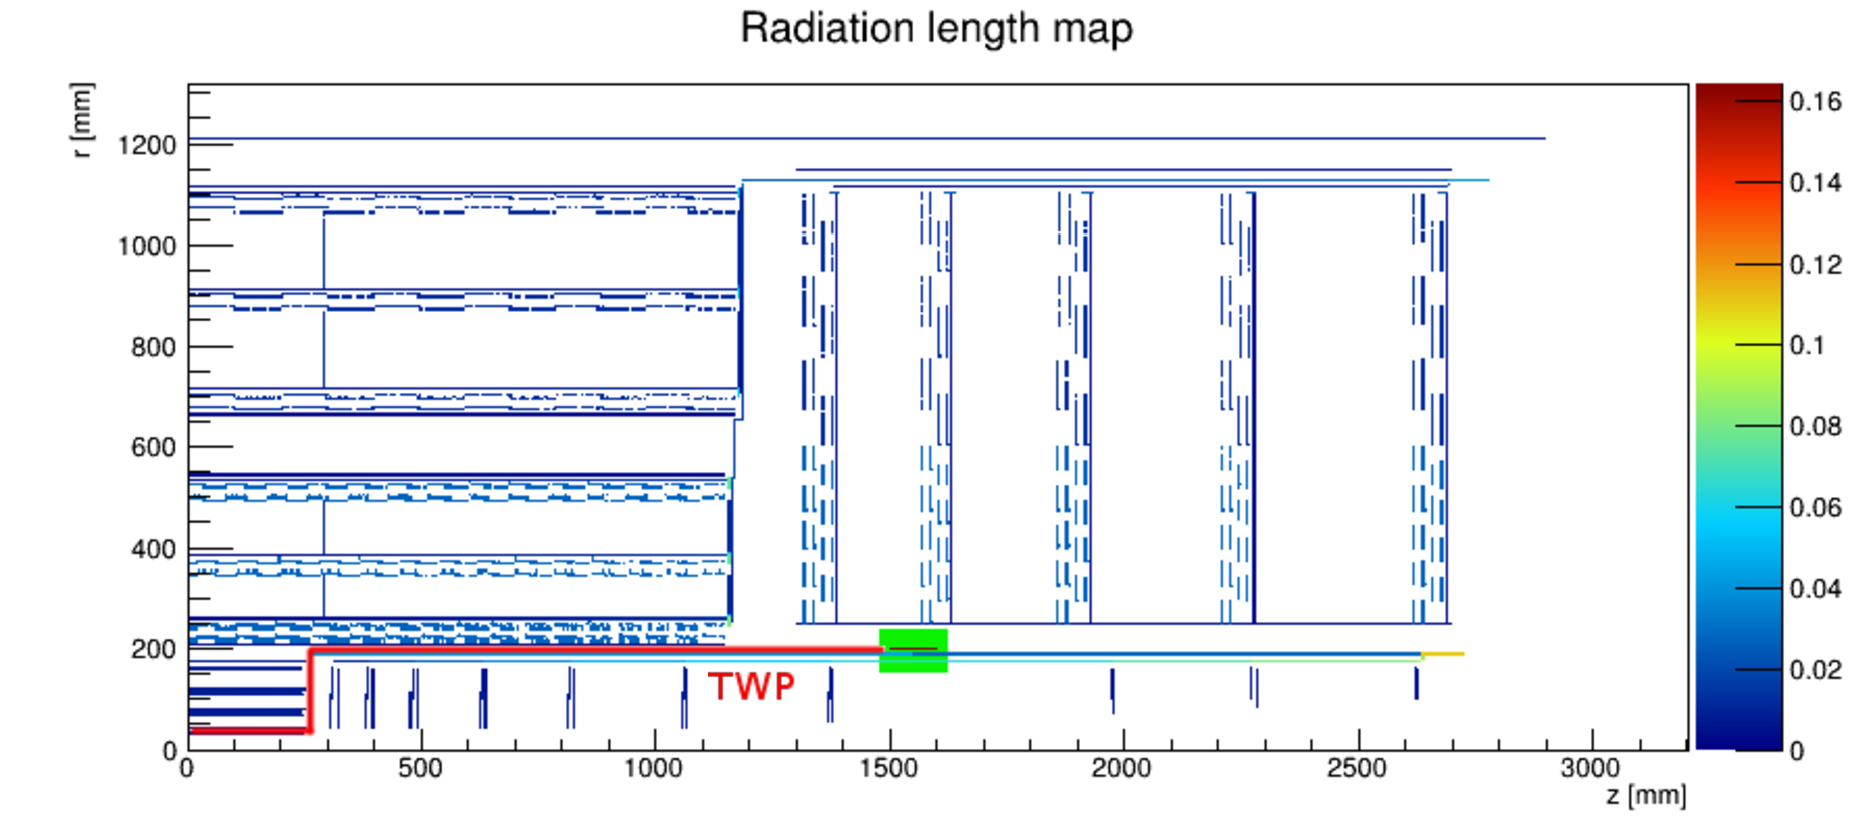
\includegraphics[width=\textwidth]{img/electro-opto2.pdf}}
    \only<3>{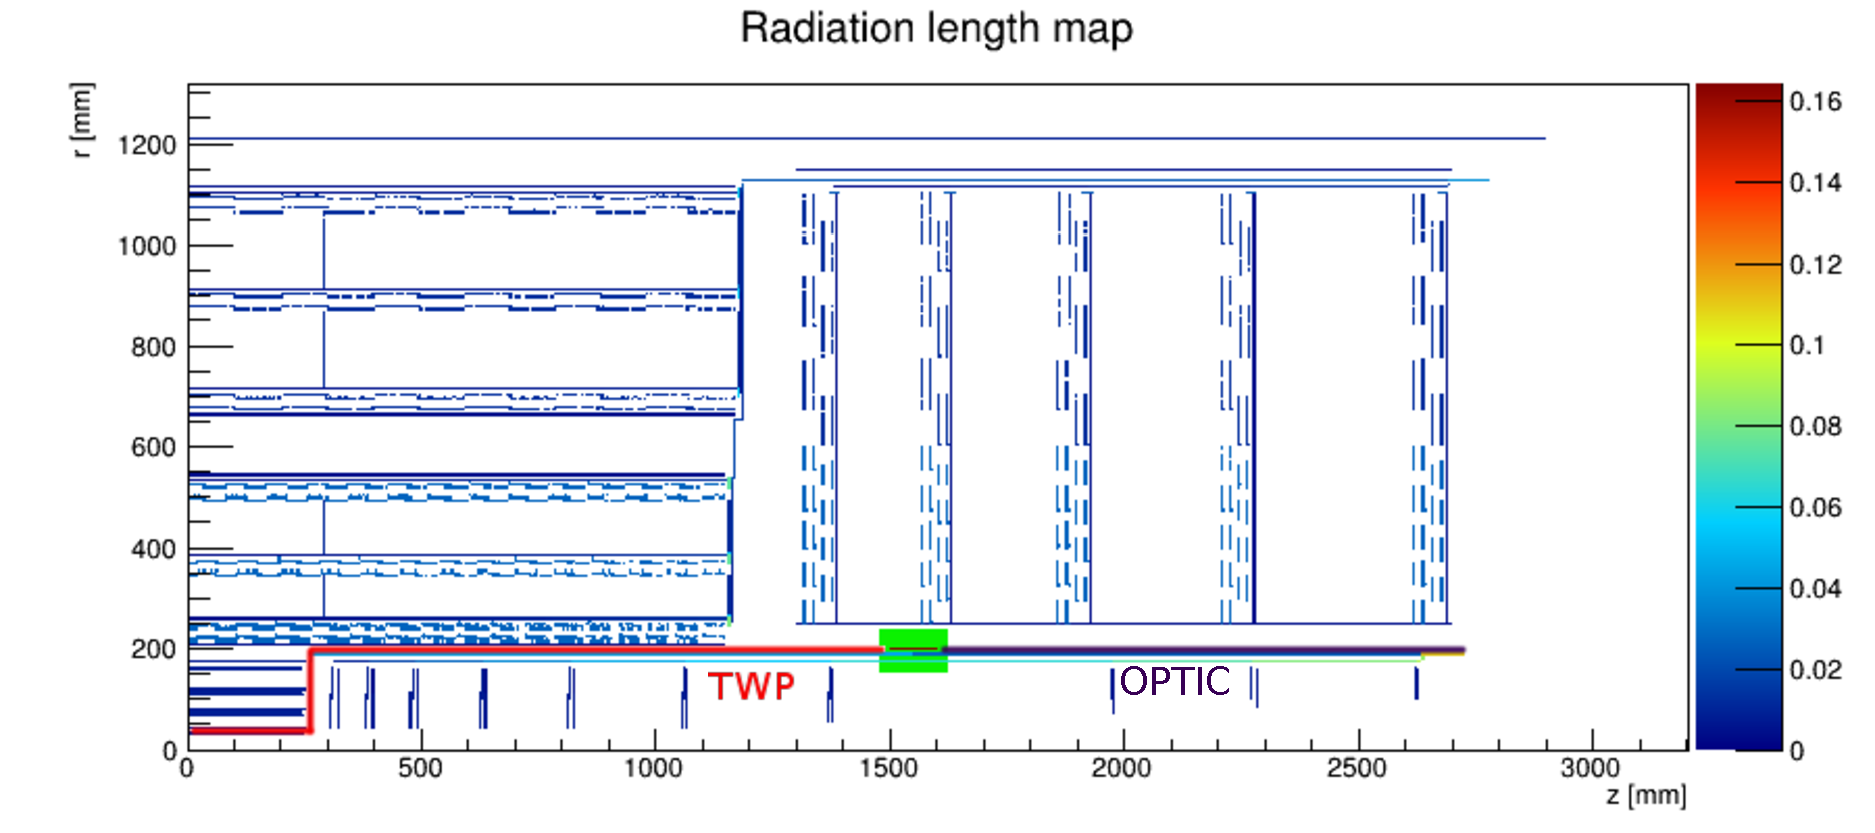
\includegraphics[width=\textwidth]{img/electro-opto3.pdf}}
  \end{center}
\end{frame}

\begin{frame}{Advantages}
  \begin{itemize}
  \item The new algorithm use the \alert{same} underlying c++ objects of the old
  \item This means that the \alert{XML} export is working as usual
    \begin{itemize}
    \item only more \alert{detailed} than before
    \end{itemize}
  \end{itemize}
\end{frame}

\begin{frame}{Validation}
  \begin{enumerate}
  \item \alert{Comparison} between old and new models
  \item Accurate \alert{tests} new model only with controlled amount of material and exact computation of material amount
  \end{enumerate}
\end{frame}

\begin{frame}{1. Comparison between old and new model \fontsize{7}{11}\selectfont (Giacomo Sguazzoni)\normalsize}
  \begin{center}
    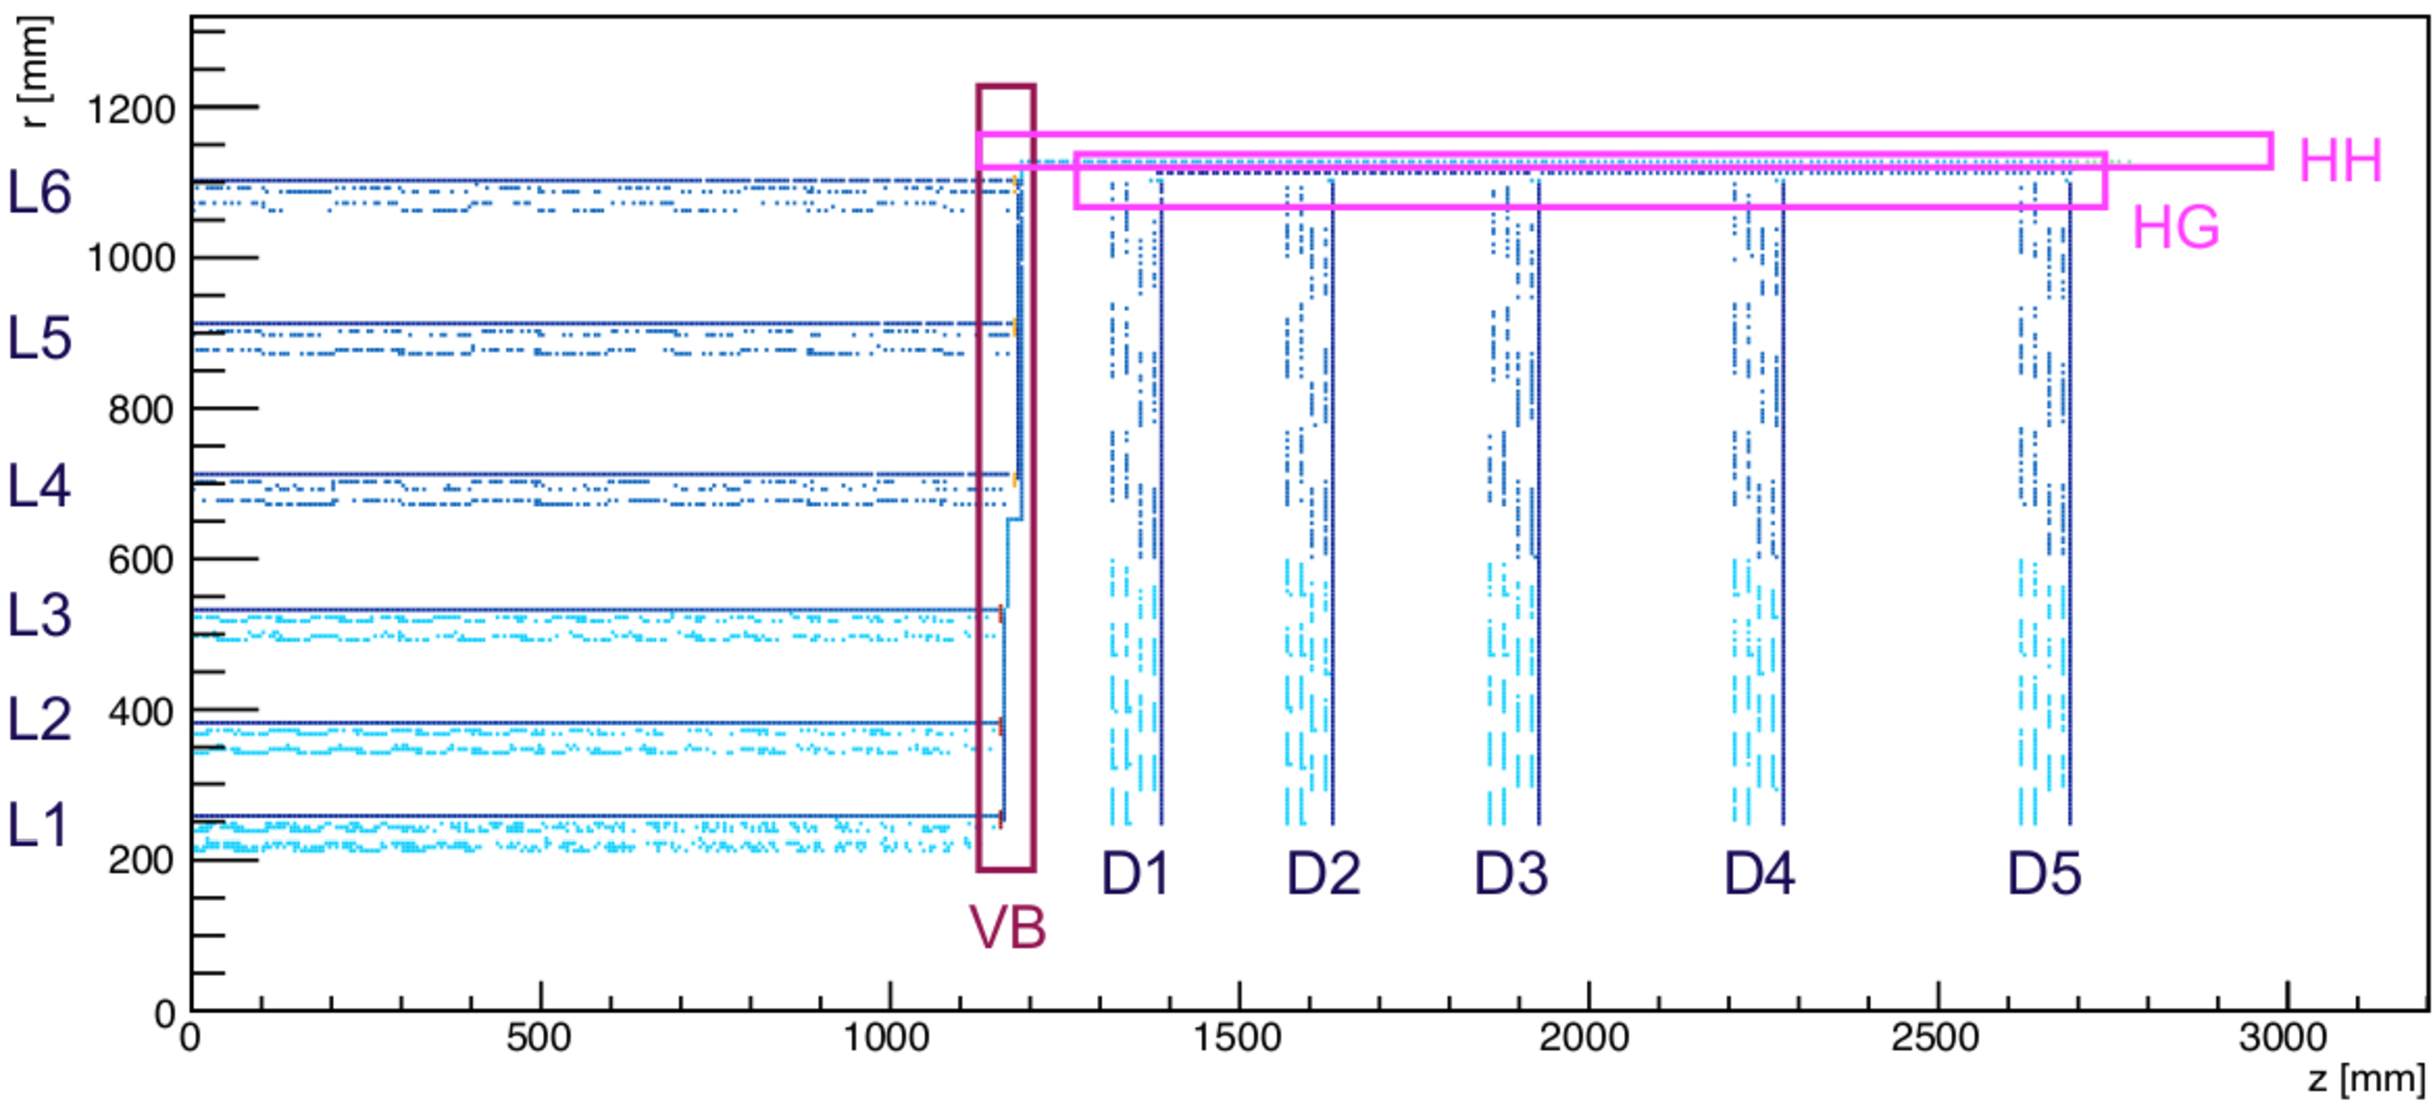
\includegraphics[width=\textwidth]{img/sguaz.pdf}
  \end{center}
\end{frame}

\begin{frame}{1. Comparison between old and new model \fontsize{7}{11}\selectfont (Giacomo Sguazzoni)\normalsize}
  \begin{center}
    \fontsize{8}{11}\selectfont
    \begin{tabular}{|c|c|c|c|c|}
      \hline
          \textbf{Area}& \textbf{New model} [g]& \textbf{Old model} [g]& \textbf{Diff.} [g]& \textbf{Diff.} [\%]\\
          \hline
          \textbf{L1}& 39871& 39665& 206& -0.5\%\\
          \hline
          \textbf{L2}& 53159& 52780& 379& -1\%\\
          \hline
          \textbf{L3}& 73872& 73643& 228&\cdots\\
          \hline
          \textbf{L4}& 51557& 49828& 1730&\\
          \hline
          \textbf{L5}& 66595& 64361& 2234&\\
          \hline
          \textbf{L6}& 81632& 78894& 2739&\\
          \hline
          \hline
          \textbf{2xD1}& 48869& 55666& -6796&\\
          \hline
          \textbf{2xD2}& 48869& 55666& -6796&\\
          \hline
          \textbf{2xD3}& 48869& 55666& -6796&\\
          \hline
          \textbf{2xD4}& 48869& 55666& -6796&\\
          \hline
          \textbf{2xD5}& 48869& 55666& -6796&\\
          \hline
          \hline
          \textbf{2xVB}& 29807& 29294& 513&\\
          \hline
          \textbf{2x(HG+HH)}& 99554& 164713& -65159&\\
          \hline
          &&&&\\
          \hline
          \textbf{Total}& 740394& 831505& -91111&\\
          \hline
          \textbf{Total (web, in kg)}& 725& 831& -106&\\
          \hline
          \textbf{Total services (web, in kg)}& 269& 194& 75&\\
          \hline
    \end{tabular}
    \normalsize
  \end{center}
\end{frame}

\begin{frame}{2. Test of new model}
  \begin{itemize}
  \item Computed the \alert{expected} material amount for given cylinders and disks of material
  \end{itemize}
  \begin{columns}
    \begin{column}{0.47\textwidth}
      \begin{block}{Cylinder, \alert{$L$} $g/mm$ of material \alert{M}}
        $$
        \frac{X_0}{X_{0M}} = \frac{L}{2\pi r \cdot X_{0M}} \cdot \frac{e^\eta+e^{-\eta}}{2}
        $$
      \end{block}
      \begin{block}{Cylinder, \alert{$L$} $mm$ of material \alert{M}}
        $$
        \frac{X_0}{X_{0M}} = \frac{L\cdot\rho_M}{X_{0M}}\cdot\frac{e^\eta+e^{-\eta}}{2}
        $$
      \end{block}
    \end{column}
    \begin{column}{0.47\textwidth}
      \begin{block}{Disk, \alert{L} $g/mm$ of material \alert{M}}
        $$
        \frac{X_0}{X_{0M}} = \frac{L}{\pi(r_1+r_2)\cdot X_{0M}}\cdot\frac{e^{2\eta}+1}{e^{2\eta}-1}
        $$
      \end{block}
      \begin{block}{Disk, \alert{$L$} $mm$ of material \alert{M}}
        $$
        \frac{X_0}{X_{0M}} = \frac{L\cdot\rho_M}{X_{0M}}\cdot\frac{e^{2\eta}+1}{e^{2\eta}-1}
        $$
      \end{block}
    \end{column}
  \end{columns}
\end{frame}

\begin{frame}{Test 1: Barrel materials}
  \begin{itemize}
  \item Built \alert{simplified} geometry
  \end{itemize}
  \begin{block}{}
    \alert{$100g/m$} of \alert{$Cu$} in each rod of each layer of pixel barrel, routed out
  \end{block}
  \begin{center}
    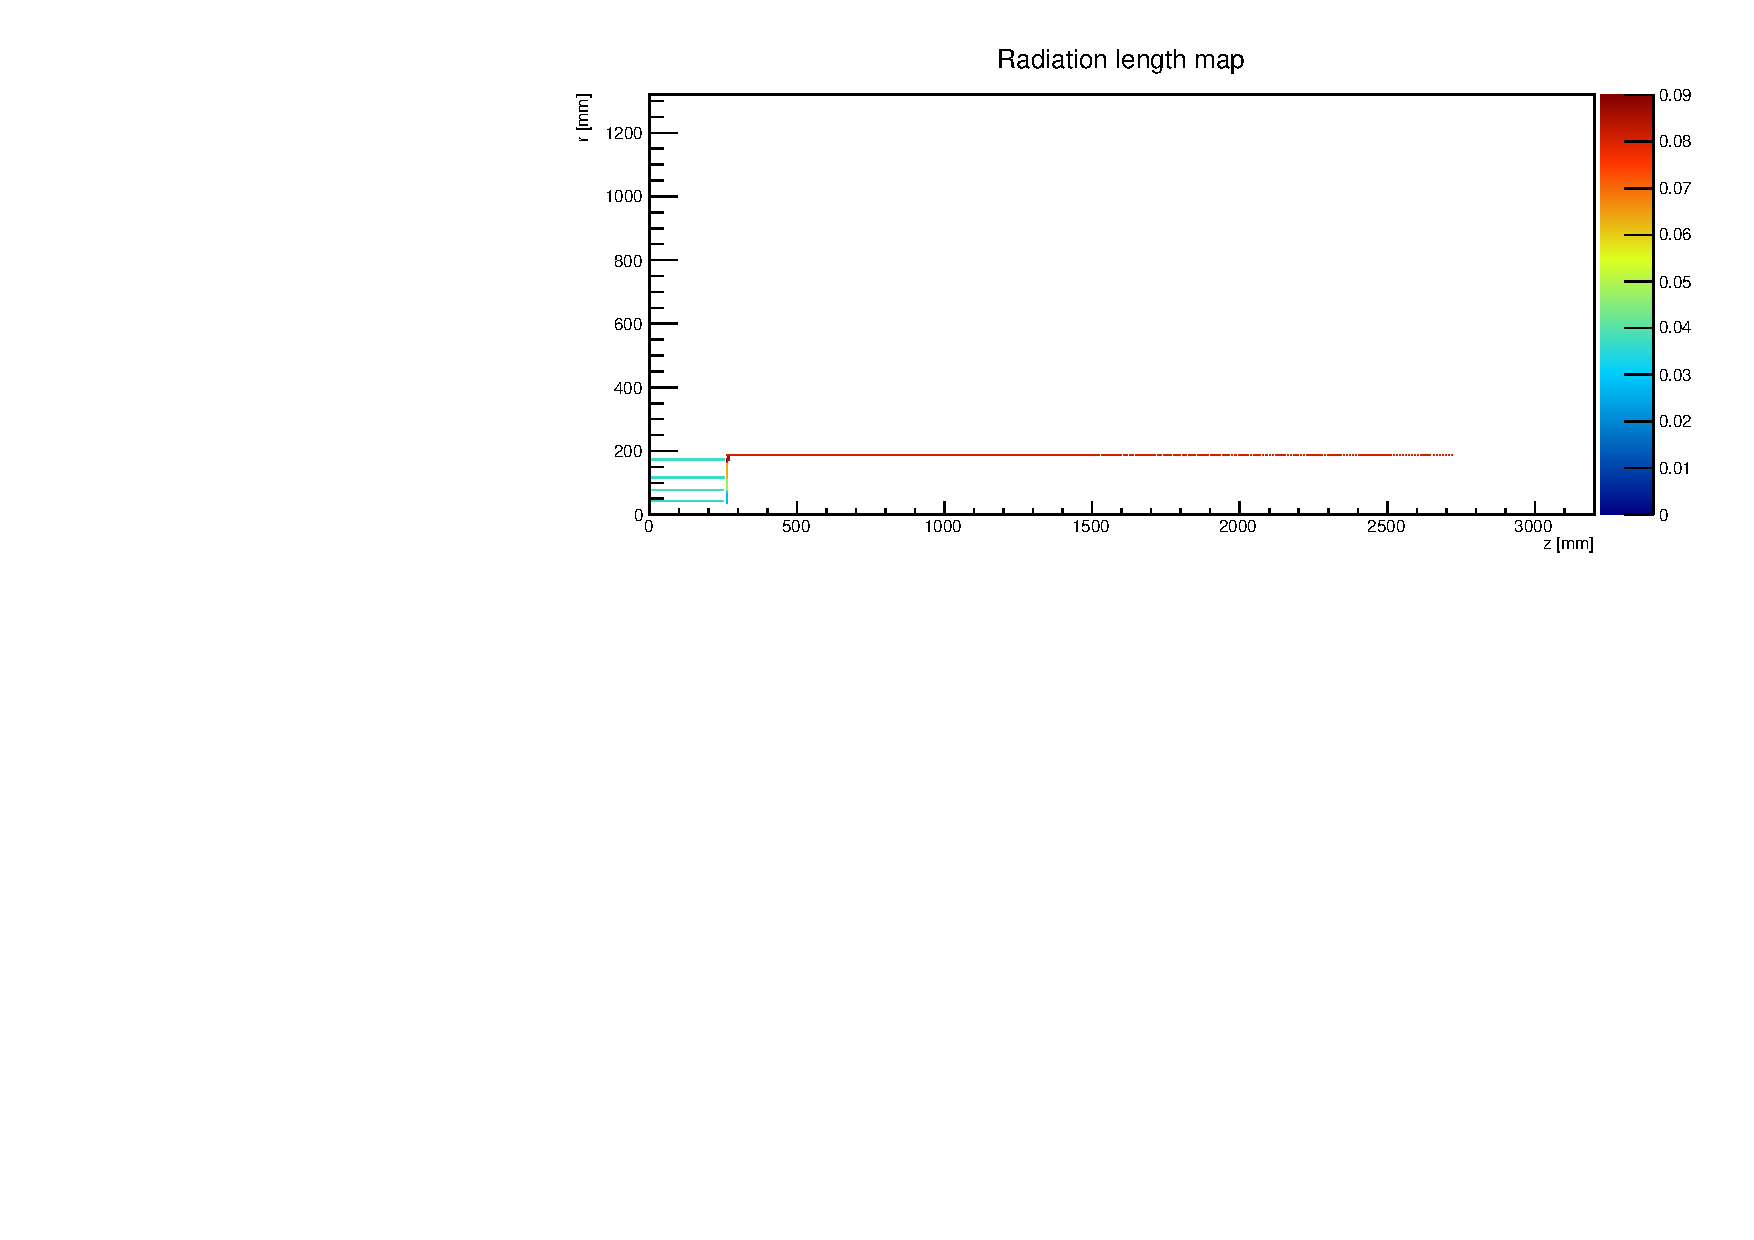
\includegraphics[width=\textwidth]{img/test2-map.pdf}
  \end{center}
\end{frame}
\begin{frame}{Test 1: Barrel materials}
  \begin{itemize}
  \item Compare \alert{computed} volumes with TkLayout's \alert{output}
  \end{itemize}
  \begin{center}
    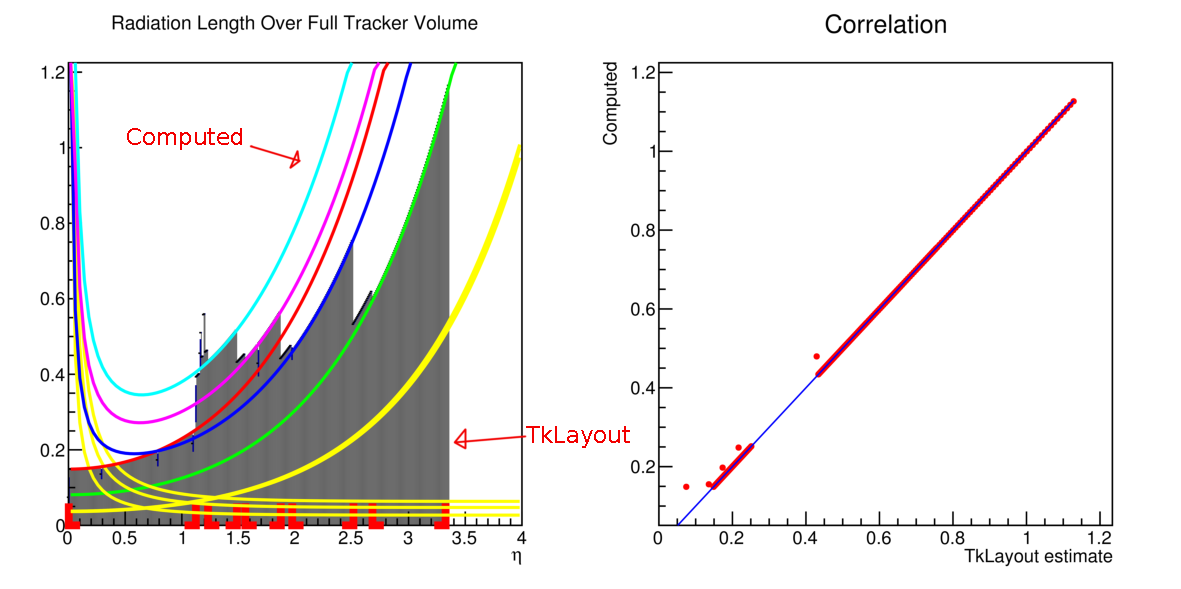
\includegraphics[width=\textwidth]{img/test2-out.pdf}
  \end{center}
\end{frame}

\begin{frame}{Test 2: Endcap materials}
  \begin{block}{}
    \alert{$100g/m$} of \alert{$Cu$} in each ``rod'' of each disk of pixel endcap, routed out
  \end{block}
  \begin{center}
    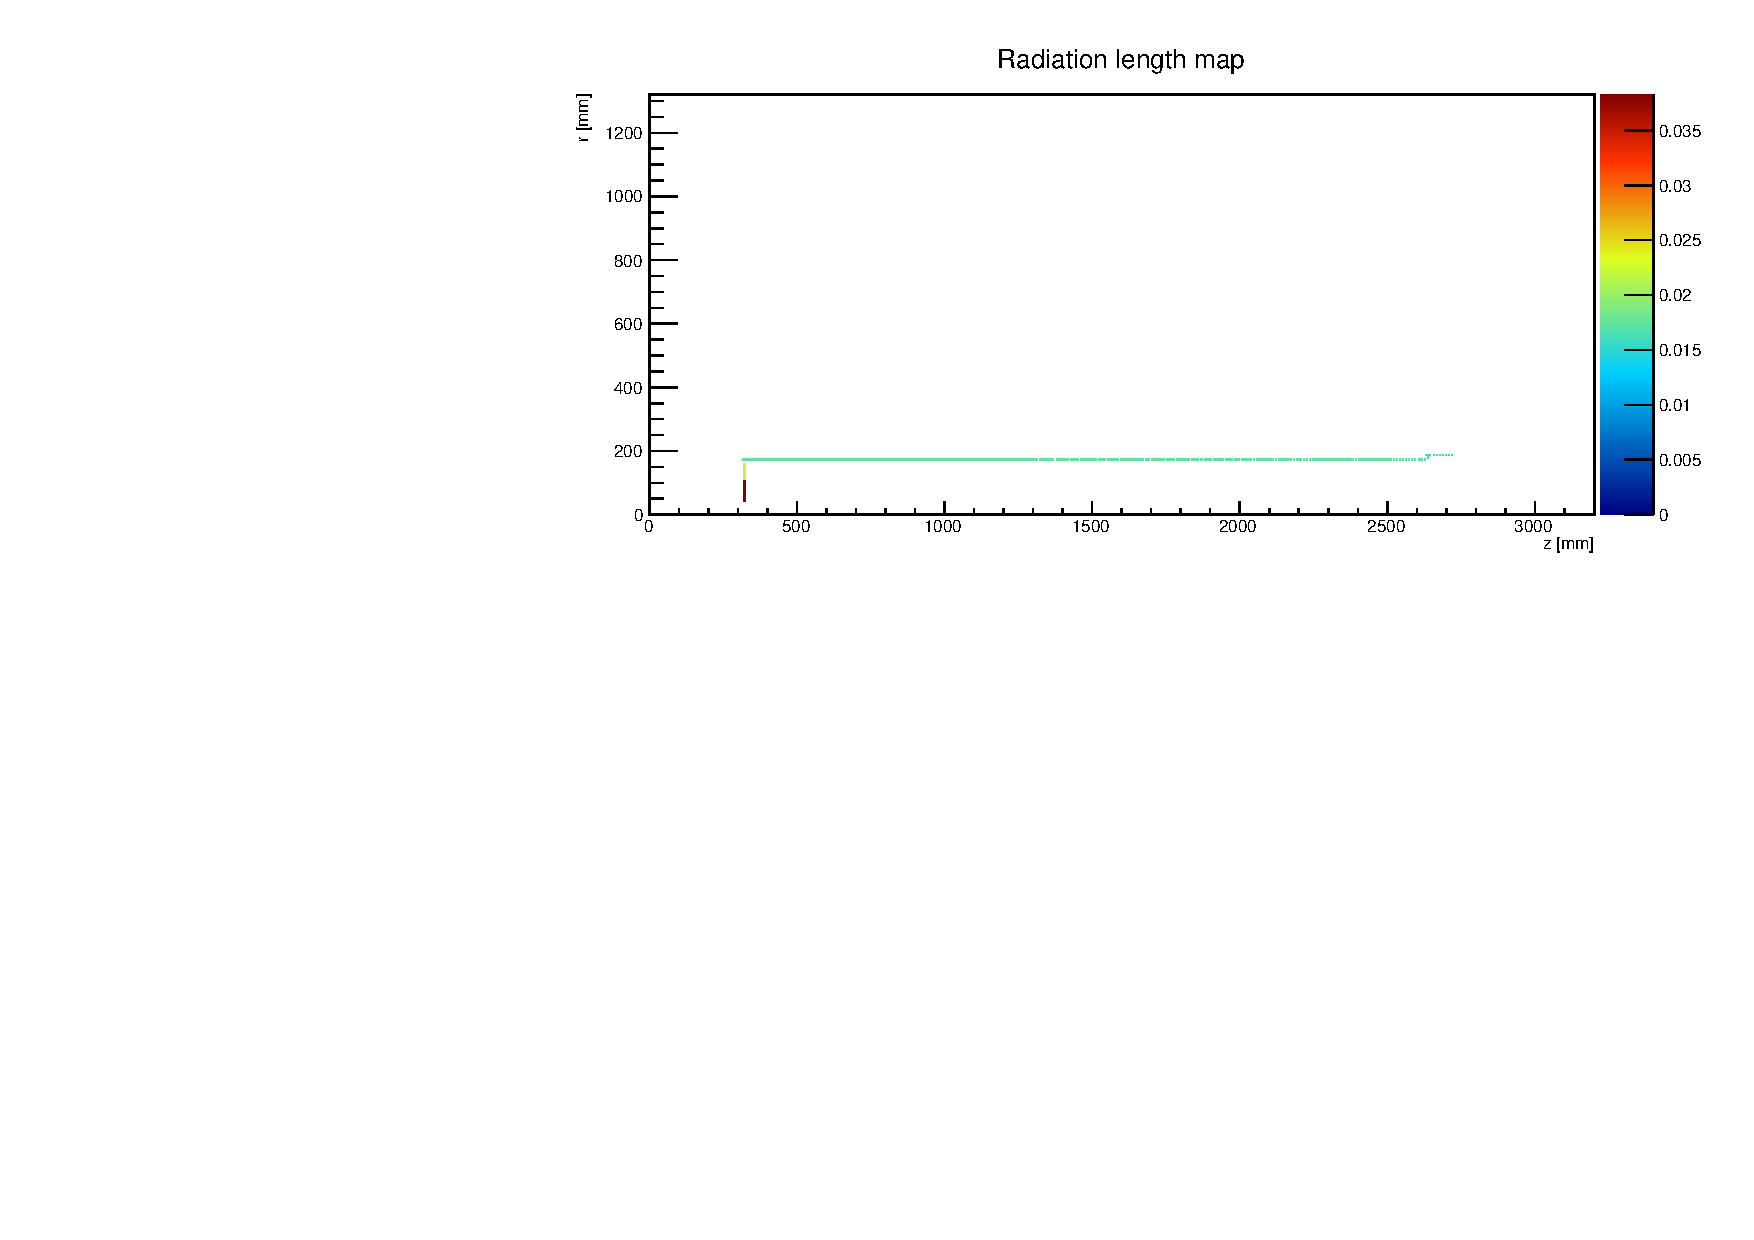
\includegraphics[width=\textwidth]{img/test6-map.pdf}
  \end{center}
\end{frame}
\begin{frame}{Test 2: Endcap materials}
  \begin{center}
    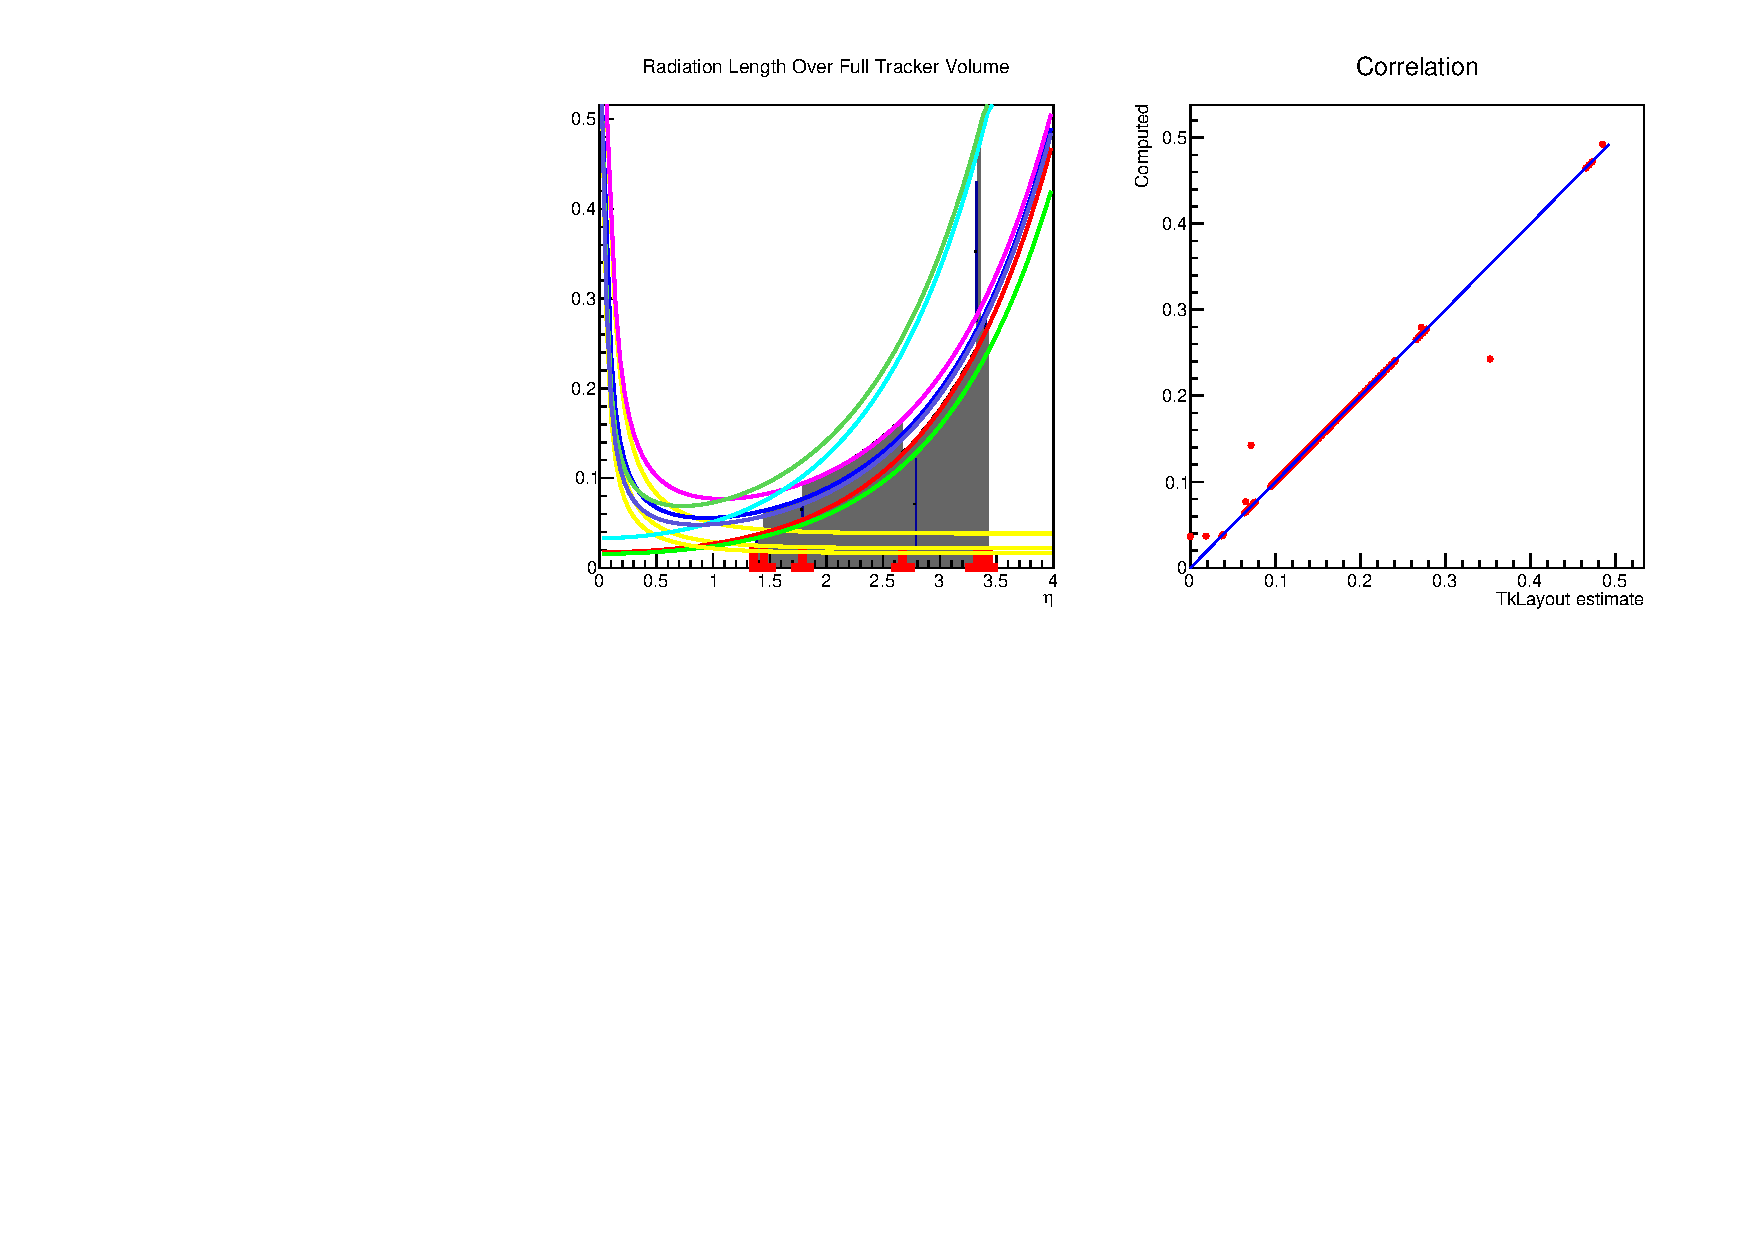
\includegraphics[width=\textwidth]{img/test6-out.pdf}
  \end{center}
\end{frame}

\begin{frame}{Module material \fontsize{7}{11}\selectfont (Ryo Yonamine)\normalsize}
\begin{enumerate}
  \item Increased level of \alert{details} for module description.
    \begin{itemize}
    \item [$\to$] \alert{4} hybrids + \alert{2} sensors + \alert{1} volume between sensors
    \end{itemize}
  \item \alert{Moved} materials out from between sensors.
    \begin{itemize}
        \item[$\to$] \alert{Less} material between sensers
        \item[$\to$] May affect rate of \alert{stubs} produced by secondary interactions
    \end{itemize}
\end{enumerate}
\begin{center}
  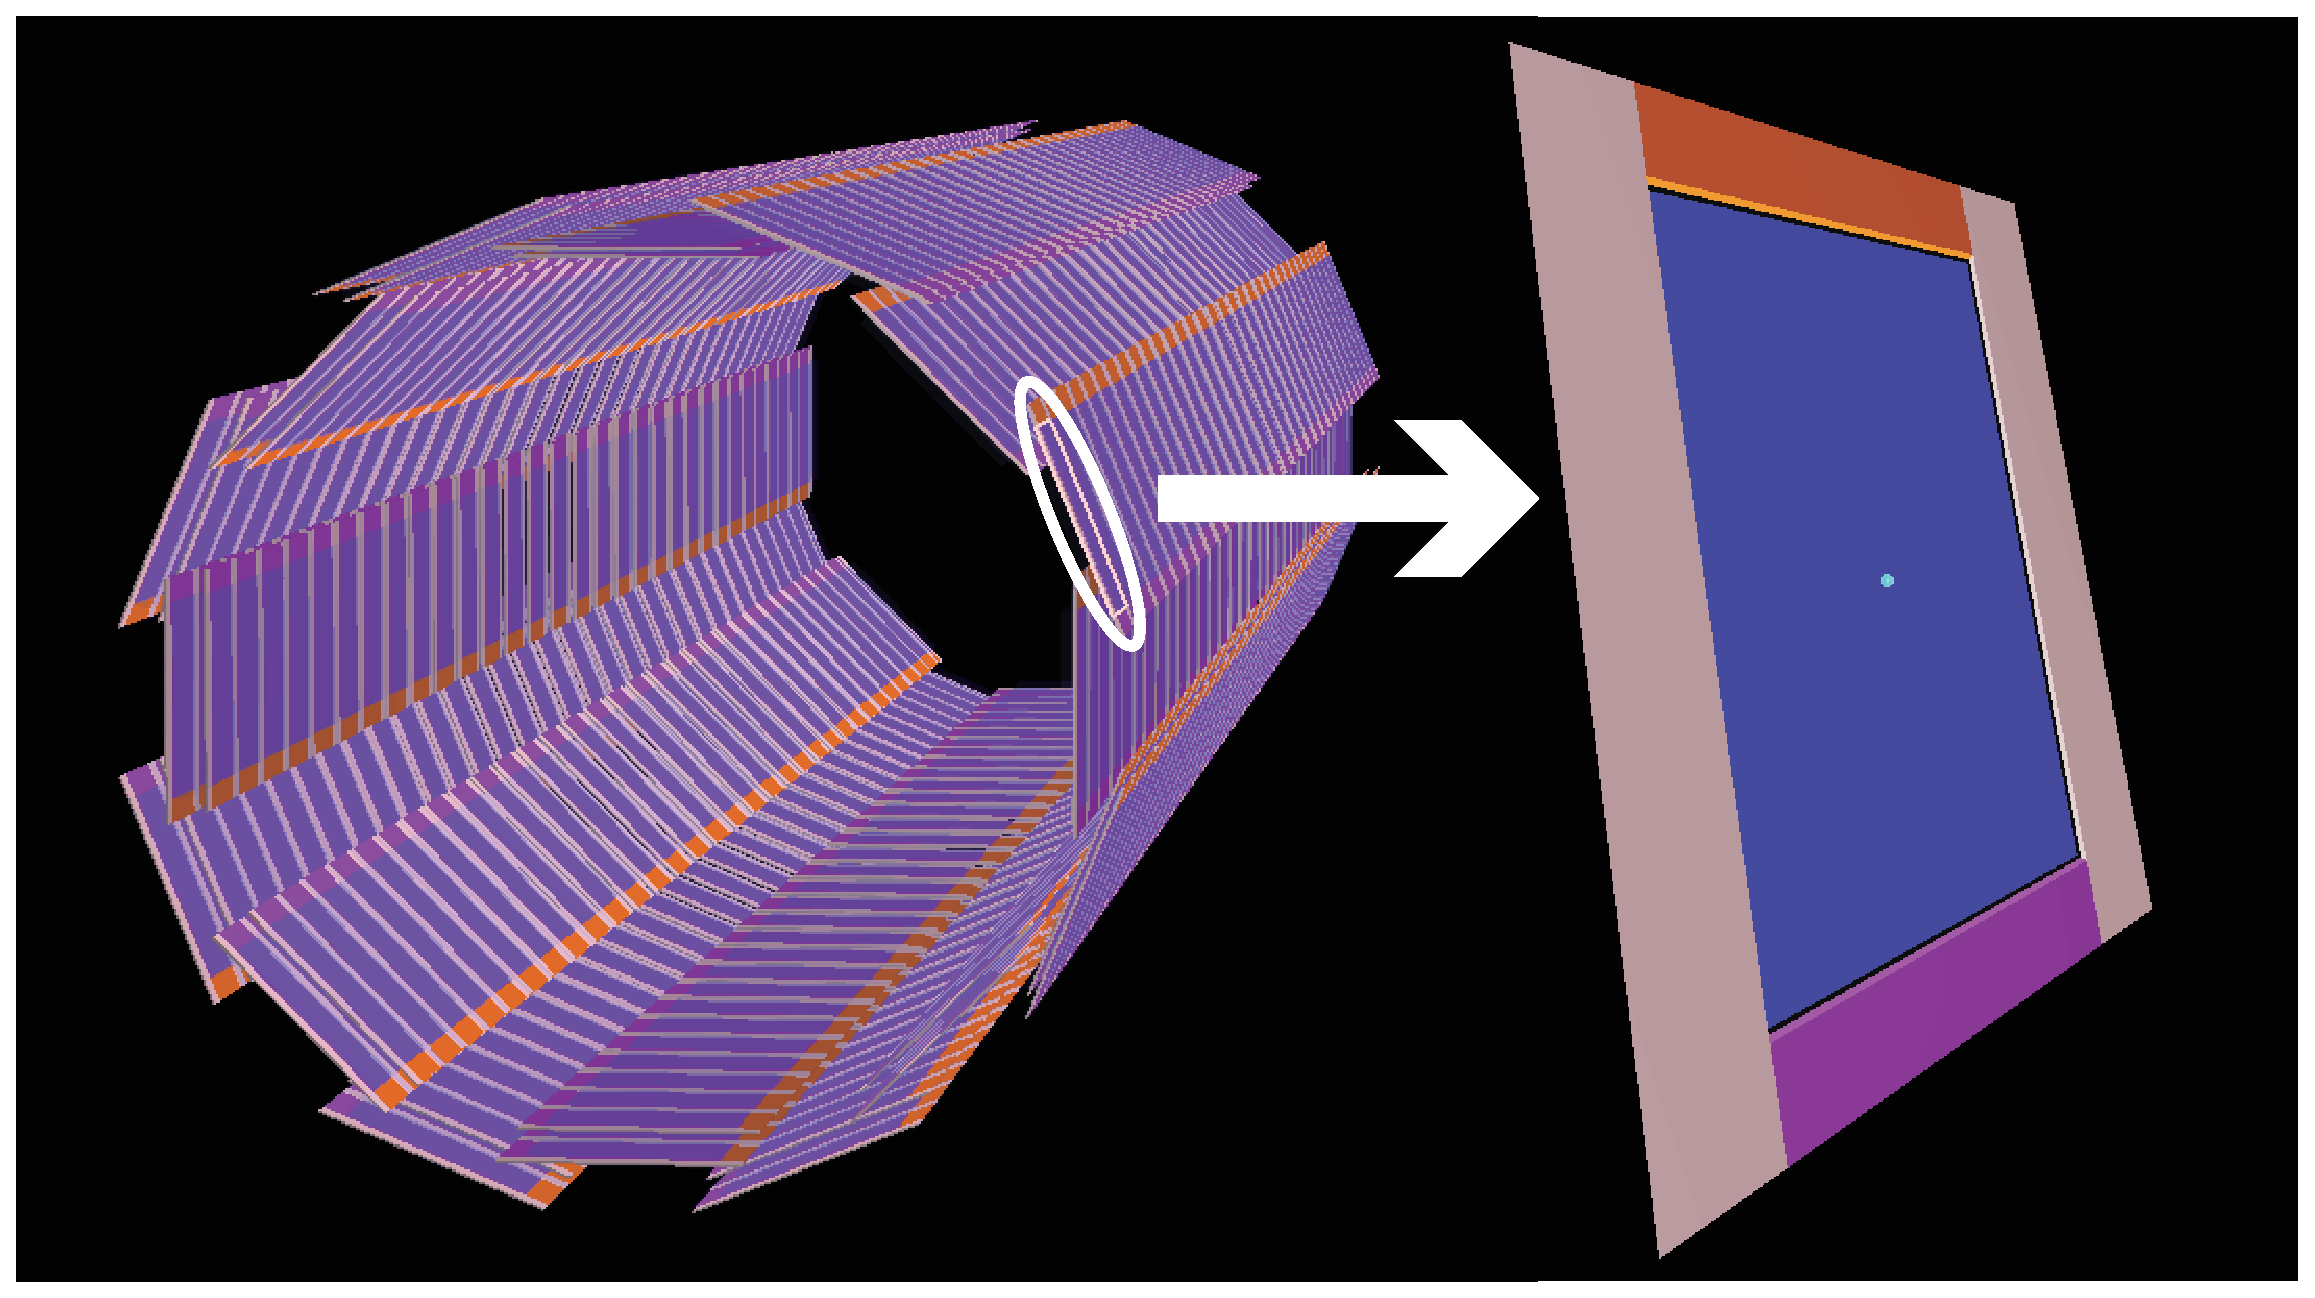
\includegraphics[width=10cm]{img/fireworks_display.eps}\\
\end{center}
\end{frame}

\begin{frame}{Preliminarily Testing XMLs in CMSSW \fontsize{7}{11}\selectfont (Ryo Yonamine)\normalsize}
  \begin{itemize}
  \item Started to \alert{compare} number of \alert{stub} with different configurations
    \begin{itemize}
    \item[$\to$] (TechProp \alert{old} material model(top-left), \alert{1\%} density material(top-right), \alert{200\%} density material(bottom-left), \alert{new} material model and output(bottom-right))
    \item T-r, b-l to \alert{quantify} the effect of change in material \alert{amount}
    \end{itemize}
  \end{itemize}
  \begin{center}
    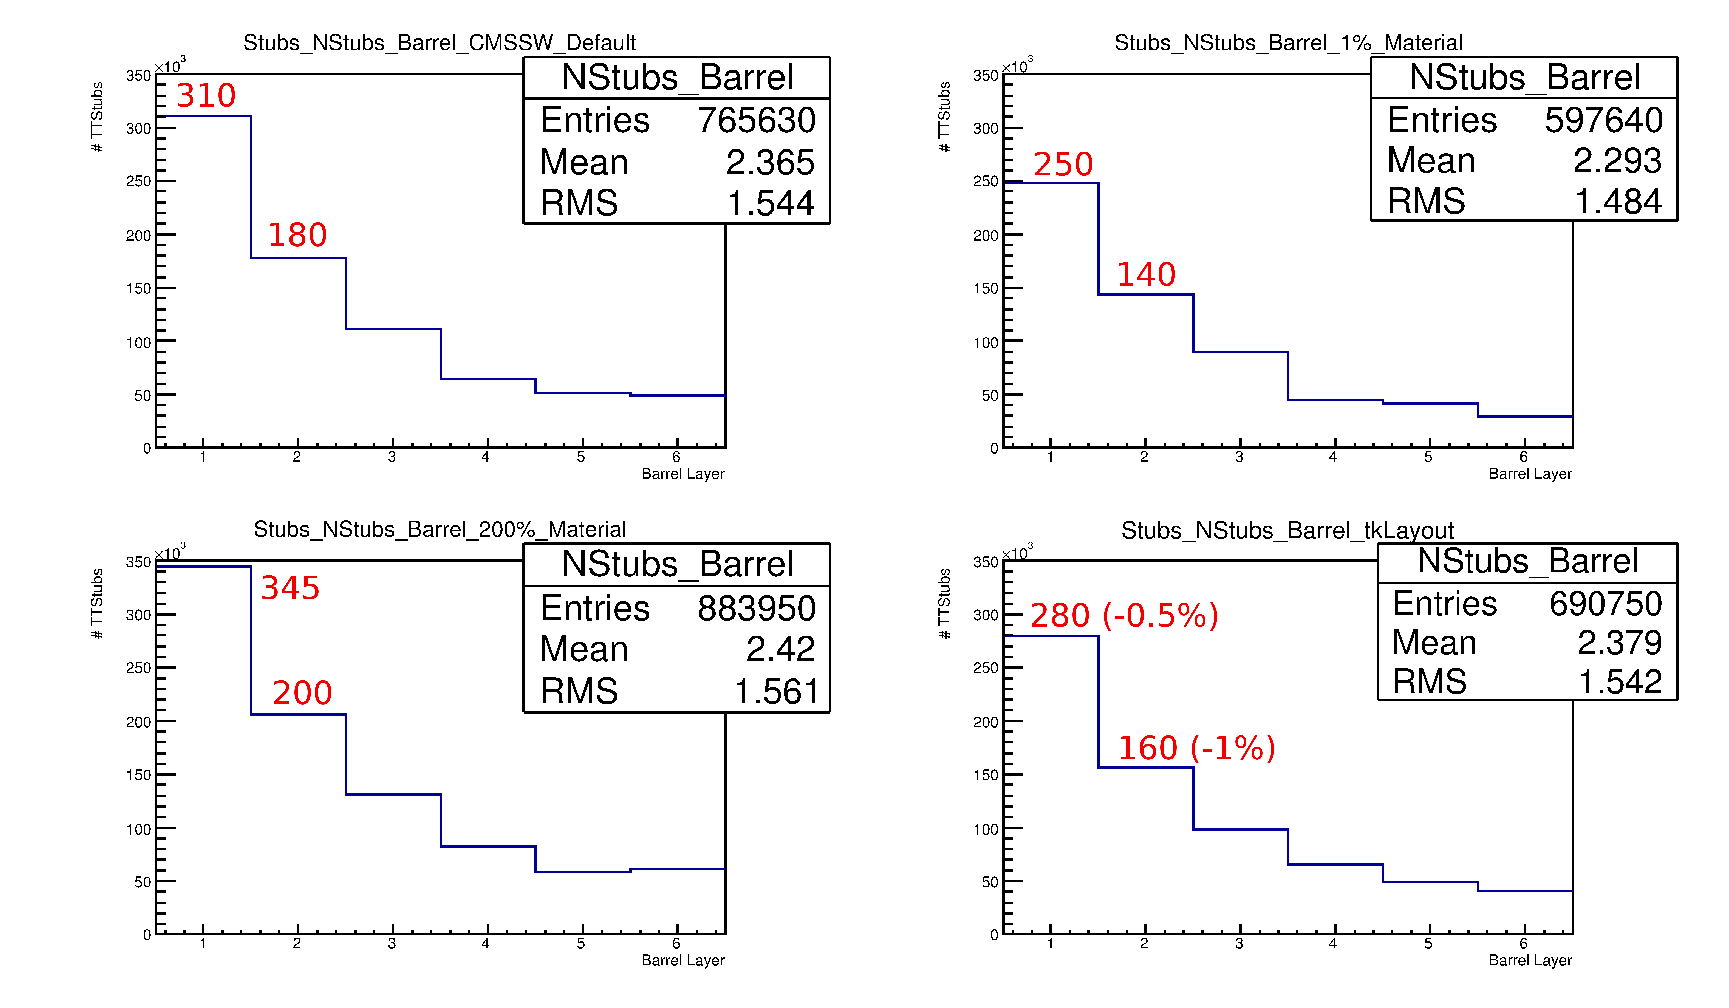
\includegraphics[width=8cm]{img/nstubs_barrel.eps}\\
  \end{center}
  \begin{itemize}
  \item Material position has a visible \alert{effect} on number of \alert{stubs}
  \end{itemize}
\end{frame}

\begin{frame}{Summary}
  \begin{enumerate}
  \item \alert{Internal}
    \begin{itemize}
    \item New material \alert{model}
    \item More \alert{precise} and \alert{detailed}
    \item New \alert{features} (pixel-alike trackers)
    \end{itemize}
  \item Working \alert{XML} export
  \item \alert{Export}
    \begin{itemize}
    \item New \alert{volumes} for outer modules (from 2+1 to 2+1+4)
    \item Just started to look for the \alert{pixel}
    \end{itemize}
  \end{enumerate}
  \begin{block}{To do}
    \begin{enumerate}
    \item Complete \alert{validation}
    \item \alert{Review} material input files with up-to-date information
    \item Complete exported \alert{XML} for pixels
    \end{enumerate}
  \end{block}
\end{frame}

\begin{frame}
  Thank you
  \begin{center}
    \fontsize{16}{11}\selectfont 
    \alert{Questions?}
    \normalsize
  \end{center}
\end{frame}

\end{document}
